\paragraph{Exercício \exno.} Segundo a Microsoft {\em Developer Network}:

\begin{itemize}
\item {\bf Índice de manutenibilidade}: Calcula um valor de índice
  entre 0 e 100 que representa a facilidade relativa de manter o
  código. Um valor alto significa a melhor manutenibilidade. As
  estimativas codificadas cor podem ser usadas para identificar
  rapidamente pontos de conflito em seu código. Uma estimativa verde
  estiver entre 20 e 100 e indica que o código tem boa a
  manutenibilidade. Uma estimativa amarela estiver entre 10 e 19 e
  indica que o código à sustentável moderadamente. Uma estimativa
  vermelha é uma estimativa entre 0 e 9 e indica pouca
  manutenibilidade.

 \item {\bf Complexidade de {\em Cyclomatic}}: Medidas a complexidade
   estrutural de código. É criado para calcular o número de diferentes
   caminhos de código no fluxo do programa. Um programa que tem o
   fluxo de controle complexo exigir mais testes obter uma boa
   cobertura de código e será menor ({\em sic}) sustentável.
\end{itemize}

Com base nas definições apresentadas, responda às seguintes questões:

\begin{enumerate}[a)]
\item Compare ou relacione as métricas apresentadas com
  as métricas de número de linhas de código e extensão ({\em coverage});

% https://msdn.microsoft.com/pt-br/library/bb385914.aspx
% https://msdn.microsoft.com/pt-br/library/ee703787.aspx

\item Algumas empresas, como a Microsoft, sugerem que a
  existência de heranças (orientação a objetos), blocos `try/catch`
  para lançamento de exceções e comandos `switch` para controle de
  fluxo podem aumentar a complexidade do código, tendo assim uma
  métrica de complexidade relacionada ao número destas
  construções. Porque estas construções podem aumentar a complexidade
  do código?
\end{enumerate}

\subsection*{Análise de ponto de função}

\Q Foi requisitado um programa para medir a condutividade de materiais
metálicos, corrente em A, em função da temperatura. Este programa
adquire valores de um multímetro, amperímetro e medidos de
temperatura. A alimentação de tensão é feita usando o método PID
(proporcional, integral, diferencial) de forma a manter constante a
variação de temperatura ao longo do tempo. O usuário deve entrar com
os dados, de acordo com a interface da Figura~\ref{fig:pidcon}.

\begin{figure}[ht]
  \centering
  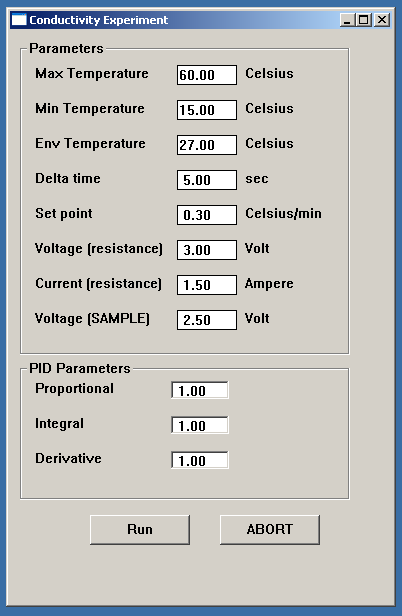
\includegraphics[scale=.3]{img/pidcon.png}
  \caption{Interface gráfica de programa para comunicação com
    instrumentos para medir condutividade de material.}
  \label{fig:pidcon}
\end{figure}

Valores de corrente e temperatura são adquiridos em um intervalo de
tempo definido pelo usuário, e armazenados em um arquivo. O gráfico de
corrente versus temperatura também deve ser confeccionado conforme o
experimento vai ocorrendo para o usuário acompanhar o experimento.
Analise a complexidade do programa utilizando a métrica de ponto de
função.

\begin{center}\footnotesize
\begin{tabular}[ht]{|l|c|c|c|c|c|}\hline
  \bf\hfil  &\bf Número de  & & & & \\
  \bf\hfil Domínio & \bf Entidades &\bf Simples &\bf Média &\bf Alta &\bf Contribuição \\\hline
  Arquivos lógicos internos (ALI) & & 7 & 10& 15 &\\\hline
  Arquivos de interface externa (AIE) & & 5 & 7 & 10 & \\\hline
  Entrada externa (EE) & & 3 & 4& 6&  \\\hline
  Saída externa (SE) &  & 4 & 5&  7& \\\hline
  Consulta externa (CE) & & 3 & 4&  6& \\\hline
\end{tabular}
\end{center}

\noindent Os pontos de função não-ajustados são \hbox{\rule{2cm}{.4pt}}.\bigskip

\begin{center}\footnotesize
        \begin{tabular}[ht]{|l|l|c|c|c|c|c|c|}\hline\hline
        \bf \hfil Características  & \bf\hfil  Nível  de &&&&&&\\
        \bf \hfil Gerais & \bf \hfil Influência & 0 & 1 & 2 & 3 & 4 & 5\\\hline
        1. Comunicação de Dados & & & & & & & \\\hline
        2. Processamento Distribuído de Dados & & & & & & &\\\hline
        3. Desempenho & & & & & & &\\\hline
        4. Configuração Intensamente Utilizada& & & & & & &\\\hline
        5. Taxa de Transação& & & & & & &\\\hline
        6. Entrada de Dados On-Line& & & & & & &\\\hline
        7. Eficiência do Usuário Final& & & & & & &\\\hline
        8. Atualização On-Line& & & & & & &\\\hline
        9. Processamento Complexo& & & & & & &\\\hline
        10. Reutilização& & & & & & &\\\hline
        11. Facilidade de Instalação& & & & & & &\\\hline
        12. Facilidade de Operação& & & & & & &\\\hline
        13. Múltiplas Localidades& & & & & & &\\\hline
        14. Facilidade de Alteração& & & & & & &\\\hline
        \bf TOTAL & & & & & & &\\\hline\hline
      \end{tabular}
\end{center}

Os pontos de ajuste são \hbox{\rule{2cm}{.4pt}}. Os pontos finais são calculados como:

\begin{center}
  pontos não-ajustados * (0,65 + 0,01*pontos de ajuste) \\\bigskip

  =\hbox{\rule{2cm}{.4pt}} * (0,65 + 0,01 * \hbox{\rule{2cm}{.4pt}}) = \hbox{\rule{2cm}{.4pt}}
\end{center}

\question{3,5} As seguintes métricas podem ser obtidas através de medidas diretas:

\begin{enumerate}[I)]
\item Tamanho do código fonte (medido pelo número de linhas);
\item Cobertura ({\em coverage}) de execução;
\item Número de defeitos ({\em bugs}) descobertos durante a realização
  de teste;
\item Tempo que um programador gasta em um projeto (medido por horas trabalhadas).
\end{enumerate}

Com base nestas métricas responda às seguintes questões:

\begin{enumerate}[a)]
\item  Qual a relação de cada uma destas métricas com a qualidade do
  sistema a ser desenvolvido? \partial{1,5}
\item Em que nível de maturidade do CMMI estas métricas seriam bem
  aproveitadas? E por quê? \partial{1,0}
\item Qual a relação, se houver, de cada uma destas métricas com a
  manutenção do código. \partial{1,0}
\end{enumerate}

\question{0,5}~{\bf Não} é considerada medida ou métrica para o monitoramento e controle do processo de desenvolvimento:

\begin{enumerate}[a)]
  \item Número de linhas de código.
  \item Análise de pontos por função.
  \item Número de caracteres do código.
  \item Extensão ({\it coverage}) do código.
  \item Densidade de defeitos do módulo.
\end{enumerate}
